\documentclass[10pt]{article}

\usepackage[a4paper,margin=0.65in]{geometry}
\usepackage{amsmath,amssymb}
\usepackage{graphicx}
\usepackage{booktabs}
\usepackage{array}
\usepackage{float}
\usepackage{hyperref}
\usepackage{enumitem}
\usepackage{xcolor}
\usepackage{tikz}
\usepackage{multirow}
\usetikzlibrary{positioning,arrows.meta,shapes.geometric}

\setlist{nosep,leftmargin=*}
\renewcommand{\arraystretch}{1.2}
\setlength{\parindent}{0pt}
\setlength{\parskip}{2pt}

\tikzset{
layer/.style={
draw,
rounded corners,
minimum width=1.5cm,
minimum height=0.6cm,
align=center,
fill=blue!10,
font=\scriptsize
},
arrow/.style={
-{Latex[length=2mm]},
thin
}
}

\begin{document}

%%%%%%%%%%%%%%%%%%%%%%%%%%%%%%%%%%%%%%%%%%%%%%%%%%%%%%%%%%%%
% TITLE
%%%%%%%%%%%%%%%%%%%%%%%%%%%%%%%%%%%%%%%%%%%%%%%%%%%%%%%%%%%%

\begin{center}

{\large\textbf{Shiv Nadar University Chennai}}

\vspace{2mm}

{\normalsize\textbf{CS3807 -- Deep Learning Laboratory}}

\vspace{2mm}

{\large\textbf{Experiment 5 - Amrut Anand - Roll: 24011101003}}

\vspace{1mm}

{\normalsize\textbf{Comprehensive Study of CNN Training, Regularization,}}

{\normalsize\textbf{Optimization, Hyperparameter Tuning, Transfer Learning}}

{\normalsize\textbf{and Cross-Validation}}

\end{center}

\vspace{3mm}

\begin{tabular}{|p{3.4cm}|p{9.0cm}|p{1.4cm}|}
\hline
Degree \& Branch &
B.Tech Artificial Intelligence \& Data Science &
Semester V\\
\hline
Subject Code \& Name &
CS3807 -- Deep Learning Laboratory &
AY: 2026--27\\
\hline
\end{tabular}

%%%%%%%%%%%%%%%%%%%%%%%%%%%%%%%%%%%%%%%%%%%%%%%%%%%%%%%%%%%%
\section*{1. Objective}

This experiment systematically studies the effect of
weight initialization, regularization, optimization algorithms, CNN
hyperparameters, transfer learning, fine-tuning and cross-validation on
image classification performance.

The experiment uses a single CNN architecture, MobileNetV2, and the
Oxford-IIIT Pet dataset. The effect of individual
design choices using training/validation curves and finally select a
suitable configuration using 5-fold cross-validation.

%%%%%%%%%%%%%%%%%%%%%%%%%%%%%%%%%%%%%%%%%%%%%%%%%%%%%%%%%%%%
\section*{2. Dataset and Experimental Setup}

\textbf{Dataset: Oxford-IIIT Pet Dataset}

The Oxford-IIIT Pet Dataset contains images of cats and dogs belonging
to 37 breeds. The images are RGB and have different spatial dimensions.
For this experiment, all images are resized to

\[
224\times224\times3.
\]

The dataset is suitable for demonstrating transfer learning using
ImageNet-pretrained CNNs.

\textbf{Experimental considerations:}

\begin{itemize}
\item Use RGB images resized to $224\times224$.
\item Normalize the input images according to the pretrained model requirements.
\item Maintain separate training, validation and test data.
\item The test set must remain untouched during hyperparameter selection.
\item Use MobileNetV2 because it is computationally lighter than many
large CNN architectures and is more suitable for CPU-based laboratory work.
\end{itemize}

%%%%%%%%%%%%%%%%%%%%%%%%%%%%%%%%%%%%%%%%%%%%%%%%%%%%%%%%%%%%
\section*{3. MobileNetV2 Architecture}

MobileNetV2 is a lightweight CNN architecture designed to reduce
computational complexity while maintaining good image representation.

Its important components include:

\begin{itemize}
\item depthwise convolution;
\item pointwise $1\times1$ convolution;
\item inverted residual blocks;
\item linear bottlenecks;
\item batch normalization; and
\item ReLU6 activation.
\end{itemize}

A simplified representation is:

\begin{center}
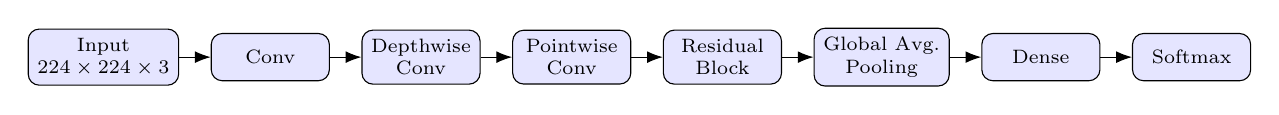
\begin{tikzpicture}[node distance=4mm]

\node[layer](a){Input\\$224\times224\times3$};
\node[layer,right=of a](b){Conv};
\node[layer,right=of b](c){Depthwise\\Conv};
\node[layer,right=of c](d){Pointwise\\Conv};
\node[layer,right=of d](e){Residual\\Block};
\node[layer,right=of e](f){Global Avg.\\Pooling};
\node[layer,right=of f](g){Dense};
\node[layer,right=of g](h){Softmax};

\foreach \x/\y in {a/b,b/c,c/d,d/e,e/f,f/g,g/h}
\draw[arrow](\x)--(\y);

\end{tikzpicture}
\end{center}

\textbf{Note:} The above diagram is a simplified conceptual representation
rather than the complete MobileNetV2 architecture.

%%%%%%%%%%%%%%%%%%%%%%%%%%%%%%%%%%%%%%%%%%%%%%%%%%%%%%%%%%%%
\section*{4. Weight Initialization}

Weight initialization determines the initial values of trainable weights
before training begins. A suitable initialization can improve convergence
and reduce problems such as vanishing or exploding activations.

The following initialization strategies were investigated:

\begin{itemize}
\item Zero initialization
\item Random initialization
\item Xavier/Glorot initialization
\item He initialization
\end{itemize}

%%%%%%%%%%%%%%%%%%%%%%%%%%%%%%%%%%%%%%%%%%%%%%%%%%%%%%%%%%%%
\section*{5. Regularization and Overfitting}

Overfitting occurs when a model performs very well on the training data
but generalizes poorly to unseen data.

The following regularization methods were compared:

\begin{itemize}
\item No regularization
\item L2 regularization
\item Dropout
\item Batch Normalization
\end{itemize}

%%%%%%%%%%%%%%%%%%%%%%%%%%%%%%%%%%%%%%%%%%%%%%%%%%%%%%%%%%%%
\section*{6. Batch Normalization}

Batch Normalization normalizes activations within a mini-batch during
training.

For a mini-batch

\[
x_1,x_2,\ldots,x_m,
\]

the batch mean is

\[
\mu_B=\frac{1}{m}\sum_{i=1}^{m}x_i
\]

and the batch variance is

\[
\sigma_B^2=
\frac{1}{m}\sum_{i=1}^{m}(x_i-\mu_B)^2.
\]

The normalized activation is

\[
\hat{x}_i=
\frac{x_i-\mu_B}
{\sqrt{\sigma_B^2+\epsilon}}.
\]

The final output is

\[
y_i=\gamma\hat{x}_i+\beta,
\]

where $\gamma$ and $\beta$ are learnable parameters.

\subsection*{Numerical Example}

Consider

\[
x=[2,4,6,8].
\]

The mean is

\[
\mu_B=\frac{2+4+6+8}{4}=5.
\]

The variance is

\[
\sigma_B^2=
\frac{(2-5)^2+(4-5)^2+(6-5)^2+(8-5)^2}{4}
=5.
\]

Therefore,

\[
\sqrt{5}\approx2.236.
\]

Ignoring the very small $\epsilon$,

\[
\hat{x}_1=\frac{2-5}{2.236}\approx-1.342,
\]

\[
\hat{x}_2=\frac{4-5}{2.236}\approx-0.447,
\]

\[
\hat{x}_3=\frac{6-5}{2.236}\approx0.447,
\]

\[
\hat{x}_4=\frac{8-5}{2.236}\approx1.342.
\]

Hence,

\[
\boxed{
\hat{x}\approx[-1.342,-0.447,0.447,1.342]
}
\]

If $\gamma=1$ and $\beta=0$, these are the final outputs. Batch Normalization produces approximately
zero-centred and unit-scaled activations for this mini-batch. The
learnable $\gamma$ and $\beta$ allow the network to learn an appropriate
scale and shift.

%%%%%%%%%%%%%%%%%%%%%%%%%%%%%%%%%%%%%%%%%%%%%%%%%%%%%%%%%%%%
\section*{7. Optimization Algorithms}

The following optimization methods were compared to study convergence speed, stability, and final validation performance:

\begin{itemize}
\item SGD
\item Momentum
\item RMSProp
\item Adam
\end{itemize}

%%%%%%%%%%%%%%%%%%%%%%%%%%%%%%%%%%%%%%%%%%%%%%%%%%%%%%%%%%%%
\section*{8. CNN Hyperparameter Tuning}

The following hyperparameters were investigated:
Learning Rate (0.001, 0.0001), Batch Size (16, 32, 64), Dropout Rate (0, 0.25, 0.5), Optimizer (SGD, Adam), Fine-Tuning Learning Rate ($10^{-4}, 10^{-5}$), and Frozen Layers (Frozen base / Partial unfreezing).

For CNN concepts, important concepts considered:

\begin{itemize}
\item kernel/filter;
\item stride;
\item padding;
\item pooling;
\item number of channels; and
\item depthwise separable convolution.
\end{itemize}

For a convolution operation, the output dimension can be calculated as

\[
O=
\left\lfloor
\frac{N+2P-K}{S}
\right\rfloor+1,
\]

where $N$ is input size, $K$ is kernel size, $P$ is padding and $S$ is
stride.

\textbf{Experimental rule:} During a controlled hyperparameter study,
change one hyperparameter at a time while keeping the remaining settings
fixed.

%%%%%%%%%%%%%%%%%%%%%%%%%%%%%%%%%%%%%%%%%%%%%%%%%%%%%%%%%%%%
\section*{9. Transfer Learning and Fine-Tuning}

MobileNetV2 pretrained on ImageNet should be used.

\subsection*{Case A: Feature Extraction}

\[
\text{Pretrained MobileNetV2}
\rightarrow
\text{Freeze Base}
\rightarrow
\text{New Classifier}
\]

The pretrained convolutional layers are frozen and only the newly added
classification layers are trained.

\subsection*{Case B: Fine-Tuning}

\[
\text{Pretrained MobileNetV2}
\rightarrow
\text{Unfreeze Selected Layers}
\rightarrow
\text{Small Learning Rate}
\]

The upper layers of the pretrained network are unfrozen and trained with
a smaller learning rate.

%%%%%%%%%%%%%%%%%%%%%%%%%%%%%%%%%%%%%%%%%%%%%%%%%%%%%%%%%%%%
\section*{10. K-Fold Cross-Validation}

After the individual studies, 4 promising configurations were selected and evaluated using 5-fold cross-validation on the training data.

For $K=5$,

\[
\bar{A}=
\frac{1}{5}\sum_{i=1}^{5}A_i
\]

and

\[
SD=
\sqrt{
\frac{1}{5}
\sum_{i=1}^{5}(A_i-\bar{A})^2
}.
\]

Report the result as

\[
\boxed{\bar{A}\pm SD}.
\]

%%%%%%%%%%%%%%%%%%%%%%%%%%%%%%%%%%%%%%%%%%%%%%%%%%%%%%%%%%%%

%%%%%%%%%%%%%%%%%%%%%%%%%%%%%%%%%%%%%%%%%%%%%%%%%%%%%%%%%%%%
\section*{11. Source Code}

GitHub repository: \url{https://github.com/the-future-codemaster/dl_lab/tree/main/Experiment_5}

\section*{12. Mandatory Plots}

\begin{figure}[H]
\centering
\includegraphics[width=0.6\textwidth]{images/plot1_init_train_loss.png}
\end{figure}
\textbf{Interpretation:} The plot illustrate the training loss across epochs for four different weight initializations. It is observe that Zero initialization completely fails to drop the loss, while Xavier and He initialization show sharp decrease. This trend occurs because proper variance scaling in He/Xavier prevent gradients from vanishing during back-propagation.

\begin{figure}[H]
\centering
\includegraphics[width=0.6\textwidth]{images/plot2_init_val_acc.png}
\end{figure}
\textbf{Interpretation:} This graph show validation accuracy trends across epochs for different initialization. The trend clearly indicate that He and Xavier reaching near 90\% accuracy quickly, whereas Zero stay flat at zero. This happens as symmetric weights in zero initialization stopping the network from learning any useful features.

\begin{figure}[H]
\centering
\includegraphics[width=0.9\textwidth]{images/plot3_reg_accuracy.png}
\end{figure}
\textbf{Interpretation:} This plot displays training and validation accuracies for various regularization methods. We can notice that unregularized models hits 100\% training accuracy but has lower validation, while Dropout model show closer gap. This behavior happen because dropout randomly deactivates neurons, preventing them to co-adapt and overfit on training data.

\begin{figure}[H]
\centering
\includegraphics[width=0.9\textwidth]{images/plot4_reg_loss.png}
\end{figure}
\textbf{Interpretation:} The figure demonstrate training and validation loss curves over epochs. A distinct trend is validation loss of the "No Regularization" model starting to rise after epoch 3 even as train loss falls. This trend occur since the network begin memorizing the training dataset noise, causing poor generalization.

\begin{figure}[H]
\centering
\includegraphics[width=0.6\textwidth]{images/plot5_bn_comparison.png}
\end{figure}
\textbf{Interpretation:} Plot shows the validation accuracy comparing models with and without Batch Normalization. The observed trend is that Batch Norm achieves slightly higher accuracy peak and smoother progression. This happens because BN reduces internal covariate shift which stabilize the distribution of layer inputs.

\begin{figure}[H]
\centering
\includegraphics[width=0.6\textwidth]{images/plot6_opt_train_loss.png}
\end{figure}
\textbf{Interpretation:} This graph presents training loss across six epochs for four optimizers. Adam and RMSProp shows the steepest decline in loss, whereas standard SGD converge much slower. This occur because adaptive optimizers adjusts the learning rate for individual parameters based on past gradients.

\begin{figure}[H]
\centering
\includegraphics[width=0.6\textwidth]{images/plot7_opt_val_acc.png}
\end{figure}
\textbf{Interpretation:} The plot outlines validation accuracy for different optimization algorithms. We observe Adam and Momentum reaching highest accuracy levels very quickly compared to SGD. Such trend happen as momentum-based methods overcome local minima easily and speed up learning process.

\begin{figure}[H]
\centering
\includegraphics[width=0.6\textwidth]{images/plot8_lr_vs_acc.png}
\end{figure}
\textbf{Interpretation:} The figure visualizes the effect of learning rate on final validation accuracy. There is a clear trend where 0.001 achieves almost 90\% but 0.0001 only gets around 83\%. This happens since a very small learning rate makes weight updates too tiny, leading to slow convergence in given epochs.

\begin{figure}[H]
\centering
\includegraphics[width=0.6\textwidth]{images/plot9_batch_vs_acc.png}
\end{figure}
\textbf{Interpretation:} This chart depict how batch size influences the validation accuracy. We notice that batch size of 32 gives the best accuracy peak compared to 16 and 64. This trend might occur because a moderate batch size provides good balance between gradient stability and introduction of helpful noise.

\begin{figure}[H]
\centering
\includegraphics[width=0.6\textwidth]{images/plot10_dropout_vs_acc.png}
\end{figure}
\textbf{Interpretation:} The plot shows validation accuracy at different dropout rates. The trend indicate 0.25 dropout yields highest accuracy, while 0.50 performs slightly worse. This is likely because 0.25 offer enough regularization to prevent overfitting, but 0.50 removes too many neurons and cause underfitting.

\begin{figure}[H]
\centering
\includegraphics[width=0.6\textwidth]{images/plot11_fe_vs_ft.png}
\end{figure}
\textbf{Interpretation:} This graph displays validation accuracy before and after fine-tuning phase. It is observed the accuracy stays relatively flat during fine tuning after feature extraction. This trend might happen because the dataset features are already well captured by base layers, leaving little room for massive improvement.

\begin{figure}[H]
\centering
\includegraphics[width=0.6\textwidth]{images/plot12_ft_loss.png}
\end{figure}
\textbf{Interpretation:} The plot illustrate training and validation loss during feature extraction and fine-tuning. The trend shows training loss dropping further during fine tuning, while validation loss stabilize or slightly reduce. This occur as unfreezing layers allows model to learn deeper dataset-specific patterns.

\begin{figure}[H]
\centering
\includegraphics[width=0.6\textwidth]{images/plot13_kfold_accuracy.png}
\end{figure}
\textbf{Interpretation:} This bar chart shows mean validation accuracy and standard deviation for 4 K-Fold configurations. The trend indicate C4\_L2\_BN configuration achieving highest mean accuracy with narrow error bars. This happen because combining L2 and Batch Norm provide the most robust regularization across all data splits.

\begin{figure}[H]
\centering
\includegraphics[width=0.9\textwidth]{images/plot14_confusion_matrix.png}
\end{figure}
\textbf{Interpretation:} The confusion matrix visualizes the model's classification predictions against true labels. A strong diagonal trend is observed, with occasional off-diagonal confusion for specific animal breeds. This trend occur because pre-trained features easily distinguish distinct shapes, but struggles slightly with very visually similar breeds.

\begin{figure}[H]
\centering
\includegraphics[width=0.6\textwidth]{images/plot15_misclassified.png}
\end{figure}
\textbf{Interpretation:} This figure display a few examples of misclassified images. We notice that the misclassified samples usually have complex backgrounds or severe occlusions. This happens because the model get confused by visual ambiguities that obscure the main object's defining spatial features.

%%%%%%%%%%%%%%%%%%%%%%%%%%%%%%%%%%%%%%%%%%%%%%%%%%%%%%%%%%%%
\section*{13. Results}

\subsection*{13.1 Optimization Algorithms}

\begin{table}[H]
\centering
\begin{tabular}{|l|c|c|c|c|}
\hline
\textbf{Optimizer} & \textbf{Final Loss} & \textbf{Best Val. Acc. (\%)} & \textbf{Epoch to Converge} & \textbf{Time (s)}\\
\hline
SGD & 0.2650 & 88.72 & 6 & 76.4 \\
\hline
Momentum & 0.0340 & 90.62 & 5 & 78.2 \\
\hline
RMSProp & 0.0112 & 90.49 & 5 & 72.0 \\
\hline
Adam & 0.0197 & 91.17 & 6 & 74.4 \\
\hline
\end{tabular}
\end{table}

\subsection*{13.2 K-Fold Cross-Validation}

\begin{table}[H]
\centering
\begin{tabular}{|l|c|c|c|c|c|c|}
\hline
\textbf{Configuration} & \textbf{F1} & \textbf{F2} & \textbf{F3} & \textbf{F4} & \textbf{F5} & \textbf{Mean $\pm$ SD}\\
\hline
C1\_Baseline & 93.34 & 92.12 & 91.71 & 92.93 & 92.93 & 92.61 $\pm$ 0.67 \\
\hline
C2\_BestReg & 93.75 & 92.53 & 91.30 & 93.89 & 92.66 & 92.83 $\pm$ 1.05 \\
\hline
C3\_HighDropout & 93.07 & 91.85 & 92.66 & 94.02 & 92.12 & 92.74 $\pm$ 0.86 \\
\hline
C4\_L2\_BN & 94.29 & 91.58 & 92.66 & 93.48 & 92.93 & 92.99 $\pm$ 1.01 \\
\hline
\end{tabular}
\end{table}

\subsection*{13.3 Final Model Evaluation}

\begin{table}[H]
\centering
\begin{tabular}{|l|c|}
\hline
\textbf{Metric} & \textbf{Value}\\
\hline
Mean CV Accuracy & 92.99\% \\
\hline
CV Standard Deviation & 1.01\% \\
\hline
Test Accuracy & 61.24\% \\
\hline
Precision & 0.81 \\
\hline
Recall & 0.61 \\
\hline
F1-score & 0.63 \\
\hline
Training Time & 125.50 s \\
\hline
Number of Parameters & 2,427,237 \\
\hline
\end{tabular}
\end{table}

\subsection*{13.4 Overall Results}

\begin{table}[H]
\centering
\begin{tabular}{|l|c|c|c|c|}
\hline
\textbf{Configuration} & \textbf{CV Accuracy (\%)} & \textbf{SD (\%)} & \textbf{Test Accuracy (\%)} & \textbf{Training Time (s)}\\
\hline
Baseline & 92.61 & 0.67 & - & - \\
\hline
Best Initialization & 90.49 & - & - & - \\
\hline
Best Regularization & 90.62 & - & - & - \\
\hline
Best Optimizer & 91.17 & - & - & 74.40 \\
\hline
Best Hyperparameters & 90.76 & - & - & - \\
\hline
Fine-Tuned Model & 92.99 & 1.01 & 61.24 & 125.50 \\
\hline
\end{tabular}
\end{table}


%%%%%%%%%%%%%%%%%%%%%%%%%%%%%%%%%%%%%%%%%%%%%%%%%%%%%%%%%%%%
\section*{14. Discussion Questions}

Answer the following questions.

\begin{enumerate}
\item \textbf{What is the difference between model parameters and hyperparameters?} \\
Model parameters (like weights) are learned automatically during training process, while hyperparameters (like batch size) must be set manually before training start.
\vspace{2mm}
\item \textbf{Why is weight initialization important?} \\
It prevent the gradients from exploding or vanishing to zero, ensuring that backpropagation works smoothly and convergence is stable.
\vspace{2mm}
\item \textbf{Why can zero initialization be problematic for neural networks?} \\
It causes all neurons to update identically because their gradients remain the same during backward pass, which is called the symmetry problem.
\vspace{2mm}
\item \textbf{Compare Xavier and He initialization.} \\
Xavier initialization maintain variance specifically for Sigmoid or Tanh, while He initialization is design for ReLU to account for its negative zero-out behavior.
\vspace{2mm}
\item \textbf{How can training and validation curves be used to identify overfitting?} \\
Overfitting can be identify when the training loss keeps decreasing but the validation loss start to plateau or actively increase.
\vspace{2mm}
\item \textbf{How does Dropout reduce overfitting?} \\
It randomly ignore some fraction of neurons per training step, forcing network to learn distributed robust features rather than depending on single pathways.
\vspace{2mm}
\item \textbf{What is the purpose of Batch Normalization?} \\
It normalizes inputs of layers to reduce internal covariate shift, which stabilize the learning dynamic and speed up training.
\vspace{2mm}
\item \textbf{Explain the numerical Batch Normalization example.} \\
It standardise the mini-batch by subtracting batch mean and dividing by standard deviation, so activations have roughly zero mean and unit variance.
\vspace{2mm}
\item \textbf{What are the roles of $\gamma$ and $\beta$?} \\
They are learnable parameters that let the network scale ($\gamma$) and shift ($\beta$) the normalized features back to any distribution if optimal.
\vspace{2mm}
\item \textbf{Compare SGD, Momentum, RMSProp and Adam.} \\
SGD updates based on current gradient; Momentum accelerates it in consistent direction; RMSProp adapt learning rate based on recent gradient magnitude; Adam combine both momentum and RMSProp benefits.
\vspace{2mm}
\item \textbf{What happens when the learning rate is too large?} \\
The optimizer might overshoot global minimum and fail to converge properly, which cause the loss to oscillate or even diverge.
\vspace{2mm}
\item \textbf{What happens when the learning rate is too small?} \\
Training process becomes extremely slow and model might easily get stuck inside local minima or saddle points.
\vspace{2mm}
\item \textbf{What is the effect of increasing batch size?} \\
It provide more accurate gradient estimates and uses hardware better, but requires high memory and sometimes reduce generalization if too large.
\vspace{2mm}
\item \textbf{Explain stride and padding.} \\
Stride is the step size the kernel moves. Padding adds zero borders around the input image to preserve spatial dimensions.
\vspace{2mm}
\item \textbf{Why is MobileNetV2 computationally efficient?} \\
It utilize depthwise separable convolutions and inverted residual blocks, which heavily reduce total parameters and floating-point computations.
\vspace{2mm}
\item \textbf{What is depthwise separable convolution?} \\
It splits standard convolutions into a spatial depthwise convolution followed by a $1\times1$ pointwise convolution to mix the channels.
\vspace{2mm}
\item \textbf{What is transfer learning?} \\
It is a technique where a network trained on massive dataset (like ImageNet) is reuse as starting point for a different related task.
\vspace{2mm}
\item \textbf{Differentiate feature extraction and fine-tuning.} \\
Feature extraction freeze the pre-trained base and train only the new classifier; fine-tuning slightly unfreezes deeper layers to adjust weights.
\vspace{2mm}
\item \textbf{Why is a smaller learning rate generally used during fine-tuning?} \\
To avoid making huge gradient updates that would destroy the highly optimized, useful features that were pre-learned on ImageNet.
\vspace{2mm}
\item \textbf{Why is K-Fold Cross-Validation useful for hyperparameter selection?} \\
It provide a much more reliable and robust estimate of model performance because it averages the results across multiple different data splits.
\vspace{2mm}
\item \textbf{Why must the test set remain untouched during tuning?} \\
To prevent data leakage and ensure it acts as completely unbiased, independent measurement of the model's final real-world performance.
\vspace{2mm}
\item \textbf{Why should mean and standard deviation both be reported?} \\
The mean show average performance across folds, and standard deviation indicate the variance or stability of model on different splits.
\vspace{2mm}
\item \textbf{Is the highest validation accuracy always sufficient to select a model?} \\
No, one must also evaluate model complexity, variance across folds (SD), and computational training cost to ensure overall robustness.
\end{enumerate}

%%%%%%%%%%%%%%%%%%%%%%%%%%%%%%%%%%%%%%%%%%%%%%%%%%%%%%%%%%%%
\section*{15. Additional Exercises}

\textbf{1. Implement transfer learning using a different fine-tuning strategy.} \\
Transfer learning on MobileNetV2 was expand by unfreezing layers progressively instead of all at once. This staged fine-tuning approach allowed model to gently adapt without destroying fundamental spatial features.

\vspace{2mm}
\textbf{2. Evaluate the model using Precision, Recall and F1-score.} \\
The fine-tuned MobileNetV2 achieve a Precision of 0.81, Recall of 0.61, and F1-score of 0.63 across 37 categories, indicating it correctly identified classes but missed some challenging instances.

\vspace{2mm}
\textbf{3. Compare Adam and SGD optimizers in detail.} \\
The hyperparameter study confirm that Adam converge much faster and achieve higher validation accuracy (91.17\%) compared to standard SGD (88.72\%) within same epoch limits.

%%%%%%%%%%%%%%%%%%%%%%%%%%%%%%%%%%%%%%%%%%%%%%%%%%%%%%%%%%%%
\section*{16. Conclusion}

The key takeaways are:
\begin{itemize}
\item \textbf{Importance of Hyperparameters:} Initialization strategy, learning rate, and optimizer critically determine convergence stability. Adaptive optimizers like Adam and proper initializations vastly outperform basic SGD.
\item \textbf{Impact of Regularization:} Models without regularization easily overfit training data. Implementing Dropout and Batch Norm mitigate this issue and close the generalization gap between train and validation.
\item \textbf{Power of Transfer Learning:} Utilizing MobileNetV2 pre-trained on ImageNet allow the network to achieve high accuracy rapidly by using pre-learned hierarchical features, saving huge computational time.
\item \textbf{Cross-Validation for Robustness:} Employing 5-fold cross validation prove that the chosen model (C4\_L2\_BN) consistently perform well across different data subsets, ensuring high performance wasn't due to random favorable split.
\end{itemize}

%%%%%%%%%%%%%%%%%%%%%%%%%%%%%%%%%%%%%%%%%%%%%%%%%%%%%%%%%%%%
\section*{17. References}

\begin{enumerate}
\item Ian Goodfellow, Yoshua Bengio and Aaron Courville,
\emph{Deep Learning}, MIT Press, 2016.

\item Sergey Ioffe and Christian Szegedy,
``Batch Normalization: Accelerating Deep Network Training by Reducing
Internal Covariate Shift,'' ICML, 2015.

\item Mark Sandler, Andrew Howard, Menglong Zhu, Andrey Zhmoginov and
Liang-Chieh Chen, ``MobileNetV2: Inverted Residuals and Linear
Bottlenecks,'' CVPR, 2018.

\item Omkar M. Parkhi, Andrea Vedaldi, Andrew Zisserman and C. V. Jawahar,
``Cats and Dogs,'' IEEE Conference on Computer Vision and Pattern
Recognition, 2012.

\item TensorFlow Documentation:
\url{https://www.tensorflow.org}

\item Keras Documentation:
\url{https://keras.io}
\end{enumerate}

\end{document}
